%\documentclass[letterpaper]{article}
\documentclass[8pt]{extarticle}
\usepackage{geometry}
\geometry{papersize={2.125in,2.75in}}

\usepackage[dvipsnames]{xcolor}
\usepackage{csquotes,tikz,microtype}
\usepackage{amsmath}
\usepackage{amsfonts}
\usepackage{amssymb}
\usepackage{amsthm}

\newtheorem{lem}{Lemma}[section]
\newtheorem{thm}[lem]{Theorem}
\newtheorem{fact}[lem]{Fact}
\newtheorem{prop}[lem]{Proposition}
\newtheorem{cor}[lem]{Corollary}

\theoremstyle{definition}
\newtheorem{defn}[lem]{Definition}
\newtheorem{rem}[lem]{Remark}
\newtheorem{example}[lem]{Example}
\newtheorem{exercise-thm}{Exercise}[section]
\newtheorem{question}{Question}

\newcommand \eps{\varepsilon}
\newcommand \ssm{\smallsetminus}
\setlength\parindent{0pt}


\begin{document}

\setcounter{page}{1}
\setcounter{section}{0}

\begin{center}
{\Large There is only one}\\
\vspace{0.5cm}
A zine for those who want to become one with one.\\
\vspace{0.5cm}
  \enquote{One One} was a racehorse, \\
  \enquote{One Two} was one too.\\
  \enquote{One One} won one race.\\
  12112
\end{center}


\newpage
\setcounter{page}{1}
\setcounter{section}{0}

\section{Motivation}

In their 1985 single, \enquote{One Vision}, 
the British rock band \textit{Queen} outlined the 
following research program:
\begin{center}
  So give me your hands, give me your hearts\\
  I'm ready!\\
  There's only one direction
  One world and one nation\\
  Yeah, one vision
\end{center}
\begin{flushright}
  \small{
  -- Queen, ``One Vision''}
\end{flushright}
%
%Today, there is only one.

\newpage
\setcounter{page}{1}
\setcounter{section}{0}

\section{Foundations}
We need some definitions:
\begin{center}
  \begin{tabular}{cc}
    \begin{minipage}{0.4\textwidth}
      For anyone,
      \begin{align*}
        1+1=1\\
        1-1=1\\
        1 \div 1=1\\
        1\times 1=1
      \end{align*}
    \end{minipage}
    &
    \begin{minipage}{0.4\textwidth}
      There is only one function, and it is $1$-to-$1$.
      \begin{align*}
        f(1) = 1
      \end{align*}
      and one relation: $1=1$
      %\begin{align*}
      %  1=1
      %\end{align*}
    \end{minipage}
  \end{tabular}
\end{center}

\newpage
\setcounter{page}{1}
\setcounter{section}{0}

\section{Calculus}

\begin{thm}
  Every sequence converges.
\end{thm}
\begin{proof}
  Consider a sequence: $1,1,\ldots$. $\forall \eps=1$, we have:
  \begin{align*}
    |1-1| = |1| = 1 = \eps
  \end{align*}
\end{proof}

\setcounter{lem}{0}
\begin{cor}
  Every series converges.
\end{cor}
This is left as an exercise to the reader.

\newpage
\setcounter{page}{1}
\setcounter{section}{0}

\section{Derivatives}
\begin{center}
  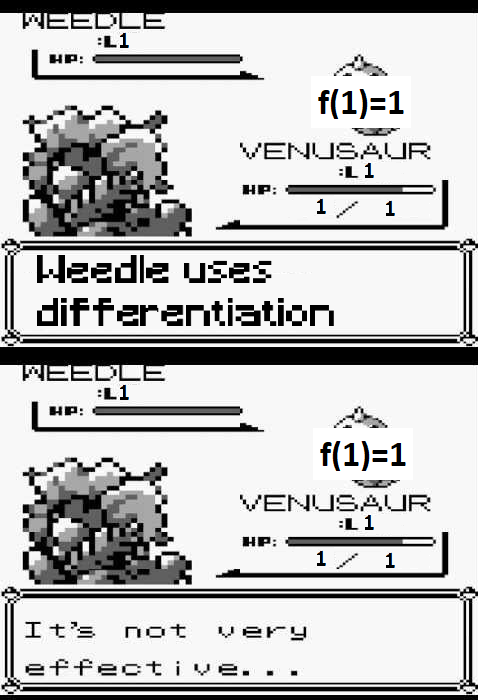
\includegraphics[width=0.55\textwidth]{differentiation.png}\\
\begin{align*}
  f'(1)&=\lim_{h\to 1}\frac{f(h)-f(1)}{h-1}=1
       %&=\lim_{1\to 1}f(1+1)-f(1)=\lim_{1\to1}1 = 1
\end{align*}
\end{center}


\newpage
\setcounter{page}{1}
\setcounter{section}{0}

\section{Topology and Geometry}
Here is a true statement:
\begin{center}
  There exist manifolds, $M^m$ and $N^n$ with $n>m$, 
  and with $N = M\ssm \{\ast\}$
\end{center}

\textbf{Q:} What do you call the empty manifold?\\
\textbf{A:} Pointless.\\
\textbf{Q:} How many covers does the empty manifold 
have with the topology?\\
\textbf{A:} One.

\begin{thm}
  Every manifold is algebraic
\end{thm}
\begin{proof}
  Every manifold can be realized as the solution set 
  to the polynomial $1=1$
\end{proof}

\newpage
\setcounter{page}{1}
\setcounter{section}{0}

\section{Complexity}
One makes computers more efficient if one 
removes the useless $0$'s between the $1$'s.\\
Here's a turing machine:
\begin{center}
  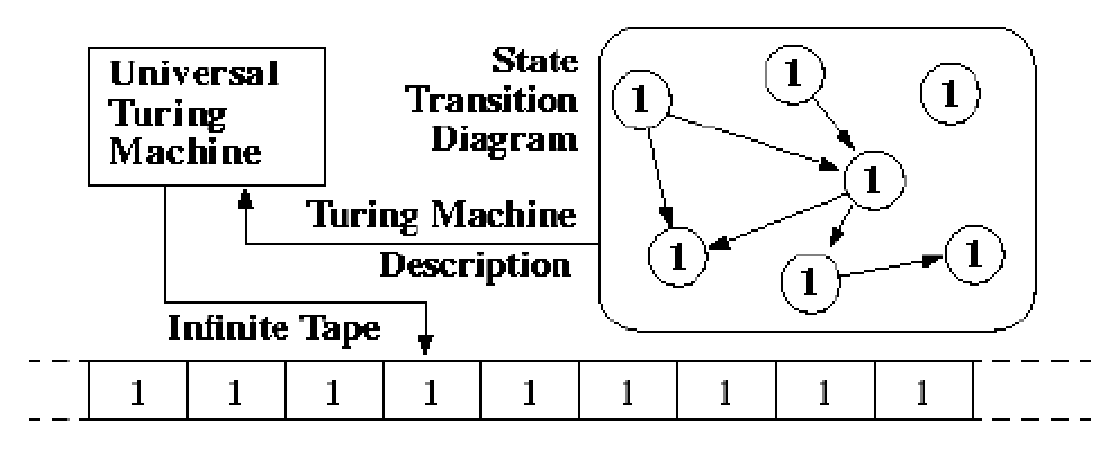
\includegraphics[width=0.9\textwidth]{turing_machine.png}
\end{center}
\begin{cor}
  The halting problem is solvable.
\end{cor}
\begin{proof}
  Halt at $1$.
\end{proof}





% draw pictures of machines whose input is something hard, and the
% output is 1.
%
% Maybe talk about halting problem?
%
%

\newpage
\setcounter{page}{1}
\setcounter{section}{0}

\section{Algebra}
There is only one group. Hey look! It's your friend group!
\begin{center}
  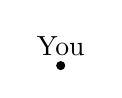
\begin{tikzpicture}[scale=0.5pt]
    \filldraw (0,0) circle (0.1);
    \node[above] at (0,0) {You};
  \end{tikzpicture}
\end{center}

There is only one ring.
\begin{center}
  \begin{tabular}{cc}
    \begin{minipage}{0.5\textwidth}
      
\includegraphics[width=0.5\textwidth]{ring.png}
    \end{minipage}
    &
    \begin{minipage}{0.5\textwidth}
      Did you miss it?\\
      Sauron sure did.
    \end{minipage}
  \end{tabular}
\end{center}

% Idea: Sauron reaching for his phone, or maybe Sauron missing the one
% ring?



\newpage
\setcounter{page}{1}
\setcounter{section}{0}

\section{The Riemann Hypothesis}
Consider the function:
\begin{align*}
  \zeta(s) = \sum \frac{1}{n^s}
\end{align*}
The above series converges, by Corollary 1.1.
We wish to find the roots of $\zeta$. That is, 
we wish to find places where $\zeta(s) = 1$. Plug in $s=1$, 
to and we're done.
\vspace{0.5cm}\\
This has many important applications in 
the distribution of the single 
prime number, $1$.

\newpage
\setcounter{page}{1}
\setcounter{section}{0}

\section{P vs. NP}
One provides a solution to 
the Boolean satisfiability 
problem.
\begin{center}
  \begin{verbatim}
  True=1, False=1
  \end{verbatim}
\end{center}
One verifies 
the satisfiability 
of any formula in $O(1)$ time.
\begin{center}
  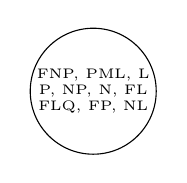
\begin{tikzpicture}[scale=0.2pt]
    \draw (0,0) circle (4);
    \node at (0,0) {\tiny P, NP, N, FL};
    \node[below] at (0,0) {\tiny FLQ, FP, NL};
    \node[above] at (0,0) {\tiny FNP, PML, L};
  \end{tikzpicture}
\end{center}

% picture of NP, P, L, etc.. complexities, but they all overlap


\newpage
\setcounter{page}{1}
\setcounter{section}{0}

\section{Algebra}
There is only one group. Hey look! It's your friend group!
\begin{center}
  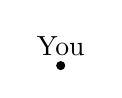
\begin{tikzpicture}[scale=0.5pt]
    \filldraw (0,0) circle (0.1);
    \node[above] at (0,0) {You};
  \end{tikzpicture}
\end{center}

There is only one ring.
\begin{center}
  \begin{tabular}{cc}
    \begin{minipage}{0.5\textwidth}
      
\includegraphics[width=0.5\textwidth]{ring.png}
    \end{minipage}
    &
    \begin{minipage}{0.5\textwidth}
      Did you miss it?\\
      Sauron sure did.
    \end{minipage}
  \end{tabular}
\end{center}

% Idea: Sauron reaching for his phone, or maybe Sauron missing the one
% ring?

\newpage
\setcounter{page}{1}
\setcounter{section}{0}

\section{Algebra}
There is only one group. Hey look! It's your friend group!
\begin{center}
  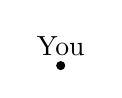
\begin{tikzpicture}[scale=0.5pt]
    \filldraw (0,0) circle (0.1);
    \node[above] at (0,0) {You};
  \end{tikzpicture}
\end{center}

There is only one ring.
\begin{center}
  \begin{tabular}{cc}
    \begin{minipage}{0.5\textwidth}
      
\includegraphics[width=0.5\textwidth]{ring.png}
    \end{minipage}
    &
    \begin{minipage}{0.5\textwidth}
      Did you miss it?\\
      Sauron sure did.
    \end{minipage}
  \end{tabular}
\end{center}

% Idea: Sauron reaching for his phone, or maybe Sauron missing the one
% ring?

\end{document}
